\documentclass[tikz,border=2pt]{standalone}
\usepackage{pgfplots}
\usepackage{libertine}
\pgfplotsset{compat=1.18}
\usetikzlibrary{arrows.meta,patterns}

\definecolor{scalarblue}{HTML}{1F6E7A}
\definecolor{projsteel}{HTML}{8A969C}
\definecolor{blindred}{HTML}{7E2F3A}
\definecolor{softgrid}{HTML}{D7DEE2}

\begin{document}
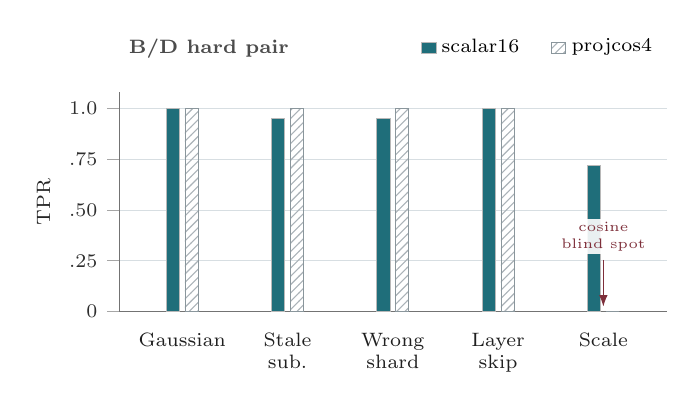
\begin{tikzpicture}
\begin{axis}[
    width=3.36in,
    height=1.72in,
    ybar,
    bar width=4.8pt,
    ymin=0,
    ymax=1.08,
    enlarge x limits=0.15,
    axis x line*=bottom,
    axis y line*=left,
    ylabel={TPR},
    ylabel style={font=\scriptsize, text=black!85},
    symbolic x coords={Gaussian,Stale,Wrong,Layer,Scale},
    xtick=data,
    xticklabels={Gaussian,{Stale\\sub.},{Wrong\\shard},{Layer\\skip},Scale},
    x tick label style={font=\scriptsize, align=center, text=black!88},
    ytick={0,0.25,0.5,0.75,1.0},
    yticklabels={0,.25,.50,.75,1.0},
    y tick label style={font=\scriptsize, text=black!82},
    tick align=outside,
    xtick style={draw=none},
    ytick style={draw=black!35, line width=0.25pt},
    axis line style={black!55, line width=0.35pt},
    ymajorgrids=true,
    major grid style={draw=softgrid, line width=0.28pt},
    legend style={
        at={(1.0,1.11)},
        anchor=south east,
        draw=none,
        fill=none,
        legend columns=2,
        font=\scriptsize,
        /tikz/every even column/.append style={column sep=0.95em}
    },
    legend image code/.code={
        \path[#1] (0cm,-0.07cm) rectangle (0.18cm,0.07cm);
    },
    clip=false,
]

\addplot+[fill=scalarblue, draw=black!28, line width=0.18pt] coordinates {
    (Gaussian,1.00)
    (Stale,0.95)
    (Wrong,0.95)
    (Layer,1.00)
    (Scale,0.72)
};
\addplot+[fill=black!5, draw=projsteel, line width=0.25pt,
          pattern=north east lines, pattern color=projsteel!72] coordinates {
    (Gaussian,1.00)
    (Stale,1.00)
    (Wrong,1.00)
    (Layer,1.00)
    (Scale,0.00)
};
\legend{scalar16, projcos4}

\node[anchor=south west, font=\scriptsize\bfseries, text=black!70]
    at (axis description cs:0.0,1.11) {B/D hard pair};
\node[anchor=south, font=\tiny, text=blindred, align=center,
      fill=white, fill opacity=0.90, text opacity=1, inner sep=1.2pt]
    at (axis cs:Scale,0.28) {cosine\\blind spot};
\draw[-{Latex[length=1.45mm]}, blindred, line width=0.36pt]
    (axis cs:Scale,0.255) -- (axis cs:Scale,0.025);

\end{axis}
\end{tikzpicture}
\end{document}
